\begin{figure}
\centering
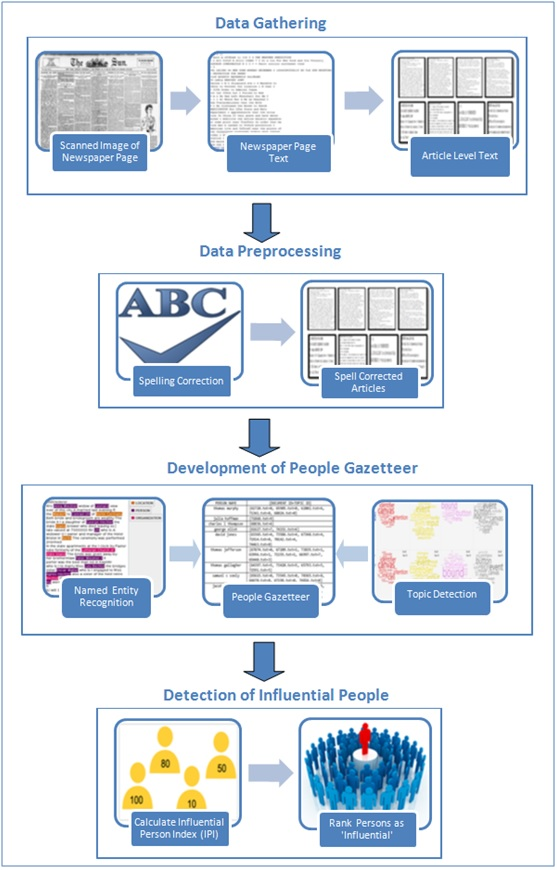
\includegraphics[width=0.5\textwidth, height=0.6\textheight]{framework4}
\caption{Research Framework showing components of proposed solution}
\label{fig:framework}
\vspace{-10pt}
\end{figure}
Figure~\ref{fig:framework} presents the framework for machine learning to aid prosopographical research. It has the following components:
%\begin{itemize}
(1)  \textbf{Data Gathering: } Prosopographical studies involve research on biographies of a group of people and is therefore severely limited by the quantity and quality of data accumulated about the past. Often in historical groups, a lot of information is available about some people, and almost nothing about some others. Studies are severely affected by lack of information and hence secondary sources of information are resorted to including demographic sources (such as parish registers), economic sources (such as deeds of sales), fiscal sources (such as tax lists), financial sources (such as city accounts), administrative sources (such as company records), religious sources (such as membership lists of fraternities), judicial sources (such as sentences), family archives and photographs, publicly available information (such as newspaper archives). The context of the research is sketched based on the available literature and has to be sufficient, relevant and easily accessible. Much debate has also gone into whether to use a single source or multiple sources. While some researchers favor verification from multiple sources, hypothesizing that a single source can lead to erroneous interpretation and one sided views of the past, others prefer a single source primarily due to the homogeneity and ease of processing the data. 

For this research, the primary source are digitized newspaper archives. In order to make a newspaper available for searching on the Internet,
the following processes \cite{dutta2011learning} must take place: (1) the microfilm copy of original paper is scanned; (2) master and Web image files are
generated; (3) metadata is assigned for each page to improve the
search capability of the newspaper; (4) OCR software is run over high
resolution images to create searchable full text and (5) OCR text,
images, and metadata are imported into a digital library software
program. 
(2) \textbf{Data Pre-processing: } The images obtained from the OCR software are segmented to obtain article level data. Both manual and automatic segmentation procedures can be used. 
%Automatic segmentation primarily involves extraction of text from images by using the logical structure of the page to produce the
%informative units -- the articles. Sometimes machine learning methods are used to label each image, then the page
%logical structure is constructed up from there by the detection of
%structuring entities such as horizontal and vertical separators, titles
%and text lines \cite{Palfray12}.
%%%%%%%%%%%%%%%%%%%%%DOUBT HERE: If we say manual segmentation, then how do we justify that segmentation on 14020 articles? 
For our work, manual segmentation is resorted to.
Following this, several preprocessing steps are applied on the text of the news
articles including  spelling correction and evaluation using a novel algorithm presented in \cite{Gupta_14a}.
%%%%%%%%%%%%%%%%%%%%%%%%%DOUBT HERE: Coreference resolution is applied after this step. Should we mention it here?
(3)  \textbf{Development of the People Gazetteer: }This component describes the process of development
of the people gazetteer which involves Named Entity Recognition (NER) in order to find person
entities. This is followed by topic detection using Latent Dirichlet Allocation (LDA) to find the primary topic(s) of news articles
and both are linked to obtain an organized structure.
(4) \textbf{Detection of Influential People: } This component defines an \textbf{Influential Person Index}
(IPI) that incorporates several criteria for identifying and ranking of influential
people. Details about IPI, ranking and final results with some case studies are discussed in Section~\ref{influential:results}.
%\end{itemize}